%! Author = rickr
%! Date = 11/27/2021
\subsection{Search strategies}
Searching strategies used in branch-and-bound algorithms determine the order in which sub-problems are explored. The three most common techniques are, depth-first search, breadth-first search, and best-first search. Each technique is well suited for a particular scenario and the choice of search strategy for a particular problem could have a significant impact on performance and/or memory requirements.
\begin{figure}[h]
	\begin{center}
		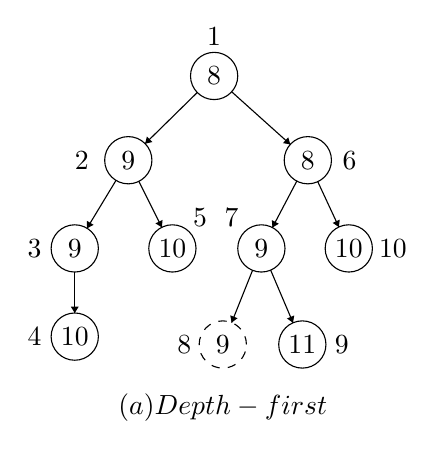
\begin{tikzpicture}[scale=0.1]
			\tikzstyle{every node}+=[inner sep=0pt]
			\draw [black] (34.8,-8) circle (3);
			\draw (34.8,-8) node {$8$};
			\draw (34.8,-3) node {$1$};
			\draw [black] (23.9,-18.7) circle (3);
			\draw (23.9,-18.7) node {$9$};
			\draw (18,-18.7) node {$2$};
			\draw [black] (46.7,-18.7) circle (3);
			\draw (46.7,-18.7) node {$8$};
			\draw (52,-18.7) node {$6$};
			\draw [black] (17.1,-29.9) circle (3);
			\draw (17.1,-29.9) node {$9$};
			\draw (12,-29.9) node {$3$};
			\draw [black] (29.5,-29.9) circle (3);
			\draw (29.5,-29.9) node {$10$};
			\draw (33,-26) node {$5$};
			\draw [black] (17.1,-41.1) circle (3);
			\draw (17.1,-41.1) node {$10$};
			\draw (12,-41.1) node {$4$};
			\draw [black] (40.8,-29.9) circle (3);
			\draw (40.8,-29.9) node {$9$};
			\draw (37,-26) node {$7$};
			\draw [black] (51.9,-29.9) circle (3);
			\draw (51.9,-29.9) node {$10$};
			\draw (57.5,-29.9) node {$10$};
			\draw [dashed] (35.9,-42.1) circle (3);
			\draw (35.9,-42.1) node {$9$};
			\draw (31,-42.1) node {$8$};
			\draw [black] (46,-42.1) circle (3);
			\draw (46,-42.1) node {$11$};
			\draw (51,-42.1) node {$9$};
			\draw [black] (32.66,-10.1) -- (26.04,-16.6);
			\fill [black] (26.04,-16.6) -- (26.96,-16.39) -- (26.26,-15.68);
			\draw [black] (37.03,-10.01) -- (44.47,-16.69);
			\fill [black] (44.47,-16.69) -- (44.21,-15.79) -- (43.54,-16.53);
			\draw [black] (22.34,-21.26) -- (18.66,-27.34);
			\fill [black] (18.66,-27.34) -- (19.5,-26.91) -- (18.64,-26.39);
			\draw [black] (25.24,-21.38) -- (28.16,-27.22);
			\fill [black] (28.16,-27.22) -- (28.25,-26.28) -- (27.35,-26.72);
			\draw [black] (17.1,-32.9) -- (17.1,-38.1);
			\fill [black] (17.1,-38.1) -- (17.6,-37.3) -- (16.6,-37.3);
			\draw [black] (39.68,-32.68) -- (37.02,-39.32);
			\fill [black] (37.02,-39.32) -- (37.78,-38.76) -- (36.85,-38.39);
			\draw [black] (41.98,-32.66) -- (44.82,-39.34);
			\fill [black] (44.82,-39.34) -- (44.97,-38.41) -- (44.05,-38.8);
			\draw [black] (45.3,-21.35) -- (42.2,-27.25);
			\fill [black] (42.2,-27.25) -- (43.01,-26.77) -- (42.13,-26.3);
			\draw [black] (47.96,-21.42) -- (50.64,-27.18);
			\fill [black] (50.64,-27.18) -- (50.75,-26.24) -- (49.85,-26.66);
			\draw (35.9,-50.1) node {$\text{(a) }Depth-first$};
		\end{tikzpicture}\qquad
		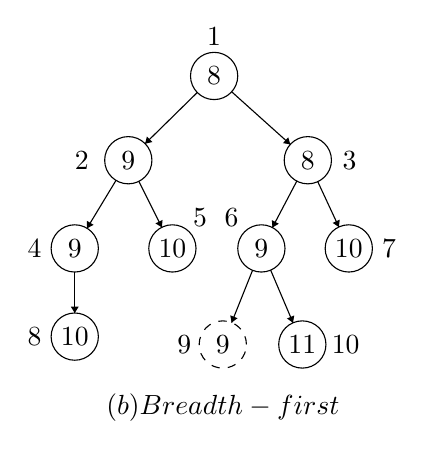
\begin{tikzpicture}[scale=0.1]
			\tikzstyle{every node}+=[inner sep=0pt]
			\draw [black] (34.8,-8) circle (3);
			\draw (34.8,-8) node {$8$};
			\draw (34.8,-3) node {$1$};
			\draw [black] (23.9,-18.7) circle (3);
			\draw (23.9,-18.7) node {$9$};
			\draw (18,-18.7) node {$2$};
			\draw [black] (46.7,-18.7) circle (3);
			\draw (46.7,-18.7) node {$8$};
			\draw (52,-18.7) node {$3$};
			\draw [black] (17.1,-29.9) circle (3);
			\draw (17.1,-29.9) node {$9$};
			\draw (12,-29.9) node {$4$};
			\draw [black] (29.5,-29.9) circle (3);
			\draw (29.5,-29.9) node {$10$};
			\draw (33,-26) node {$5$};
			\draw [black] (17.1,-41.1) circle (3);
			\draw (17.1,-41.1) node {$10$};
			\draw (12,-41.1) node {$8$};
			\draw [black] (40.8,-29.9) circle (3);
			\draw (40.8,-29.9) node {$9$};
			\draw (37,-26) node {$6$};
			\draw [black] (51.9,-29.9) circle (3);
			\draw (51.9,-29.9) node {$10$};
			\draw (57,-29.9) node {$7$};
			\draw [dashed] (35.9,-42.1) circle (3);
			\draw (35.9,-42.1) node {$9$};
			\draw (31,-42.1) node {$9$};
			\draw [black] (46,-42.1) circle (3);
			\draw (46,-42.1) node {$11$};
			\draw (51.5,-42.1) node {$10$};
			\draw [black] (32.66,-10.1) -- (26.04,-16.6);
			\fill [black] (26.04,-16.6) -- (26.96,-16.39) -- (26.26,-15.68);
			\draw [black] (37.03,-10.01) -- (44.47,-16.69);
			\fill [black] (44.47,-16.69) -- (44.21,-15.79) -- (43.54,-16.53);
			\draw [black] (22.34,-21.26) -- (18.66,-27.34);
			\fill [black] (18.66,-27.34) -- (19.5,-26.91) -- (18.64,-26.39);
			\draw [black] (25.24,-21.38) -- (28.16,-27.22);
			\fill [black] (28.16,-27.22) -- (28.25,-26.28) -- (27.35,-26.72);
			\draw [black] (17.1,-32.9) -- (17.1,-38.1);
			\fill [black] (17.1,-38.1) -- (17.6,-37.3) -- (16.6,-37.3);
			\draw [black] (39.68,-32.68) -- (37.02,-39.32);
			\fill [black] (37.02,-39.32) -- (37.78,-38.76) -- (36.85,-38.39);
			\draw [black] (41.98,-32.66) -- (44.82,-39.34);
			\fill [black] (44.82,-39.34) -- (44.97,-38.41) -- (44.05,-38.8);
			\draw [black] (45.3,-21.35) -- (42.2,-27.25);
			\fill [black] (42.2,-27.25) -- (43.01,-26.77) -- (42.13,-26.3);
			\draw [black] (47.96,-21.42) -- (50.64,-27.18);
			\fill [black] (50.64,-27.18) -- (50.75,-26.24) -- (49.85,-26.66);
			\draw (35.9,-50.1) node {$\text{(b) }Breadth-first$};
		\end{tikzpicture}\qquad
		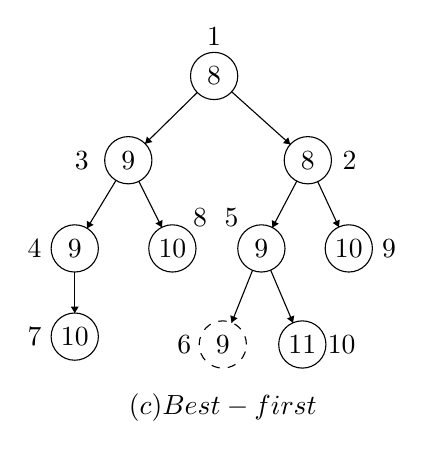
\begin{tikzpicture}[scale=0.1]
			\tikzstyle{every node}+=[inner sep=0pt]
			\draw [black] (34.8,-8) circle (3);
			\draw (34.8,-8) node {$8$};
			\draw (34.8,-3) node {$1$};
			\draw [black] (23.9,-18.7) circle (3);
			\draw (23.9,-18.7) node {$9$};
			\draw (18,-18.7) node {$3$};
			\draw [black] (46.7,-18.7) circle (3);
			\draw (46.7,-18.7) node {$8$};
			\draw (52,-18.7) node {$2$};
			\draw [black] (17.1,-29.9) circle (3);
			\draw (17.1,-29.9) node {$9$};
			\draw (12,-29.9) node {$4$};
			\draw [black] (29.5,-29.9) circle (3);
			\draw (29.5,-29.9) node {$10$};
			\draw (33,-26) node {$8$};
			\draw [black] (17.1,-41.1) circle (3);
			\draw (17.1,-41.1) node {$10$};
			\draw (12,-41.1) node {$7$};
			\draw [black] (40.8,-29.9) circle (3);
			\draw (40.8,-29.9) node {$9$};
			\draw (37,-26) node {$5$};
			\draw [black] (51.9,-29.9) circle (3);
			\draw (51.9,-29.9) node {$10$};
			\draw (57,-29.9) node {$9$};
			\draw [dashed] (35.9,-42.1) circle (3);
			\draw (35.9,-42.1) node {$9$};
			\draw (31,-42.1) node {$6$};
			\draw [black] (46,-42.1) circle (3);
			\draw (46,-42.1) node {$11$};
			\draw (51,-42.1) node {$10$};
			\draw [black] (32.66,-10.1) -- (26.04,-16.6);
			\fill [black] (26.04,-16.6) -- (26.96,-16.39) -- (26.26,-15.68);
			\draw [black] (37.03,-10.01) -- (44.47,-16.69);
			\fill [black] (44.47,-16.69) -- (44.21,-15.79) -- (43.54,-16.53);
			\draw [black] (22.34,-21.26) -- (18.66,-27.34);
			\fill [black] (18.66,-27.34) -- (19.5,-26.91) -- (18.64,-26.39);
			\draw [black] (25.24,-21.38) -- (28.16,-27.22);
			\fill [black] (28.16,-27.22) -- (28.25,-26.28) -- (27.35,-26.72);
			\draw [black] (17.1,-32.9) -- (17.1,-38.1);
			\fill [black] (17.1,-38.1) -- (17.6,-37.3) -- (16.6,-37.3);
			\draw [black] (39.68,-32.68) -- (37.02,-39.32);
			\fill [black] (37.02,-39.32) -- (37.78,-38.76) -- (36.85,-38.39);
			\draw [black] (41.98,-32.66) -- (44.82,-39.34);
			\fill [black] (44.82,-39.34) -- (44.97,-38.41) -- (44.05,-38.8);
			\draw [black] (45.3,-21.35) -- (42.2,-27.25);
			\fill [black] (42.2,-27.25) -- (43.01,-26.77) -- (42.13,-26.3);
			\draw [black] (47.96,-21.42) -- (50.64,-27.18);
			\fill [black] (50.64,-27.18) -- (50.75,-26.24) -- (49.85,-26.66);
			\draw (35.9,-50.1) node {$\text{(c) } Best-first$};
		\end{tikzpicture}\qquad
	\end{center}
	\caption{Sub-tree traversals for different searching techniques. The numbers on the side of each node correspond to the lower-bound at that step and the dotted node represents the optimal solution \cite{morrison2016branch}.}
	\label{fig:searchTechniques}
\end{figure}
\subsubsection{Depth-first}
The depth-first search strategy follows a last-in, first-out order and is implemented by maintaining a list of unexplored nodes in a stack as shown in Figure \ref{fig:searchTechniques} (a). The routine removes the top element from the stack to explore for the next sub-problem and the children generated are inserted on the top of the stack. The potential memory requirements needed to maintain a list of children nodes can become a problem, however we remedy this by maintaining a path of indices from the root to the current node instead of the entire list of unexplored sub-problems. When the current sun-problem is complete, the algorithm selects the next unexplored node for exploration and if one does not exist, the algorithm backtracks to the nearest ancestor node. The biggest issue with this technique is that it is blind to the structure of the problem and makes no use of the lower bounds encountered during a traversal. This can cause the algorithm to spend large amounts of time exploring unpromising regions, especially when the search space is unbalanced. This results in a running time of $\Theta (V+E)$ \cite{cormen2009introduction}, however DFE yields valuable information about the structure of a graph.
\subsubsection{Breadth-first}
The breadth-first search strategy, shown in Figure \ref{fig:searchTechniques} (b), explores nodes based on a first-in, first-out order and is implemented by maintaining a queue data structure. This results in the algorithm exploring all nodes at the same level before moving on to deeper portions of the tree. The advantage of this technique is that if the optimal solution is close to the root, or the tree is unbalanced, breadth-first search will find the solution faster that depth-first. However, if the solution occurs at lower depths, breadth-first can require large amounts of memory because it does not take advantage of any pruning rules. The BFS technique runs on a running time of $O(V+E)$ \cite{cormen2009introduction} and is linear to the size of an adjacency list representation of the graph.
\subsubsection{Best-first}